
\newif\ifcmt\cmtfalse

\documentclass[tikz]{standalone}

\begin{document}

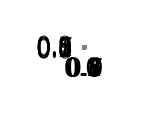
\begin{tikzpicture}
    \node[anchor=south west,inner sep=0] (image) at (0,0) {
\ifcmt
img_begin 
	any
	tags astro,galaxy
	width 0.5
img_end
\fi
		};
    \begin{scope}[x={(image.south east)},y={(image.north west)}]
        \draw[help lines,xstep=.1,ystep=.1] (0,0) grid (1,1);
        \foreach \x in {0,1,...,9} { \node [anchor=north] at (\x/10,0) {0.\x}; }
        \foreach \y in {0,1,...,9} { \node [anchor=east] at (0,\y/10) {0.\y}; }
    \end{scope}
\end{tikzpicture}
\end{document}
